\documentclass[12pt, letterpaper]{report}
\usepackage[margin=1in]{geometry}
\usepackage[utf8]{inputenc}
\usepackage{graphicx}
\usepackage{float}
\usepackage{xcolor}
\graphicspath{ {./img/} }
\setlength\parindent{0pt}
\renewcommand{\thesection}{\Roman{section}.}
\renewcommand{\thesubsection}{\alph{subsection}.}


\title{CS1555 - Serialization}
\author{Zachary M. Mattis}


\begin{document}

\maketitle

\section{History 1}


\[ H_1 = \color{red} RL_1(x), R_1(x), WL_1(x), W_1(x), \color{blue} RL_2(y), R_2(y), RU_2(y), \color{red} WL_1(y), \color{blue} C_2, \color{red} W_1(y), WU_1(x), WU_1(y), C_1 \]


\begin{table}[H]
	\centering
	\setlength\tabcolsep{4pt}
	\begin{minipage}{0.48\textwidth}
		\centering
		\begin{tabular}{ |r|r|r| }
			\hline
			& \textbf{$T_1$} & \textbf{$T_2$} \\
			\hline
			\textbf{1} & RL(x) & \\
			\hline
			\textbf{2} & R(x) & \\
			\hline
			\textbf{3} & WL(x) & \\
			\hline
			\textbf{4} & W(x) & \\
			\hline
			\textbf{5} & & RL(y) \\
			\hline
			\textbf{6} & & R(y) \\
			\hline
			\textbf{7} & & RU(y) \\
			\hline
			\textbf{8} & WL(y) & \\
			\hline
			\textbf{9} & & C \\
			\hline
			\textbf{10} & W(y) & \\
			\hline
			\textbf{11} & WU(x) & \\
			\hline
			\textbf{12} & WU(y) & \\
			\hline
			\textbf{13} & C & \\
			\hline
		\end{tabular}
		\caption{Concurrent History 1}
	\end{minipage}
	\hfill
	\begin{minipage}{0.48\textwidth}
	\centering
	\begin{tabular}{ |r|r|r| }
		\hline
		& \textbf{$T_1$} & \textbf{$T_2$} \\
		\hline
		\textbf{1} & & RL(y) \\
		\hline
		\textbf{2} & & R(y) \\
		\hline
		\textbf{3} & & RU(y) \\
		\hline
		\textbf{4} & & C \\
		\hline
		\textbf{5} & RL(x) & \\
		\hline
		\textbf{6} & R(x) & \\
		\hline
		\textbf{7} & WL(x) & \\
		\hline
		\textbf{8} & W(x) & \\
		\hline
		\textbf{9} & WL(y) & \\
		\hline
		\textbf{10} & W(y) & \\
		\hline
		\textbf{11} & WU(x) & \\
		\hline
		\textbf{12} & WU(y) & \\
		\hline
		\textbf{13} & C & \\
		\hline
	\end{tabular}
	\caption{Serial History 1}
	\end{minipage}
\end{table}


\begin{figure}[H]
	\centering
	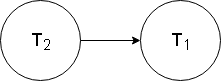
\includegraphics[width=0.5\columnwidth]{h1.png}
	\caption{SG($H_1$)}
\end{figure}


\textbf{2PL:}
\\ \\
History 1 above follows 2PL as each transaction adheres to the concurrency protocol by following both the \textit{growing} and \textit{shrinking} phases.

\pagebreak
\section{History 2}

\[ H_2 = \color{red} WL_1(x), W_1(x), WU_1(x), \color{green} RL_3(y), R_3(y), \color{blue} WL_2(x), W_2(x), WU_2(x), C_2, \color{red} C_1, \color{green} RU_3(y), C_3 \]



\begin{table}[H]
	\centering
	\setlength\tabcolsep{4pt}
	\begin{minipage}{0.48\textwidth}
		\centering
		\begin{tabular}{ |r|r|r|r| }
			\hline
			& \textbf{$T_1$} & \textbf{$T_2$} & \textbf{$T_3$} \\
			\hline
			\textbf{1} & WL(x) & & \\
			\hline
			\textbf{2} & W(x) & & \\
			\hline
			\textbf{3} & WU(x) & & \\
			\hline
			\textbf{4} & & & RL(y) \\
			\hline
			\textbf{5} & & & R(y) \\
			\hline
			\textbf{6} & & WL(x) & \\
			\hline
			\textbf{7} & & W(x) & \\
			\hline
			\textbf{8} & & WU(x) & \\
			\hline
			\textbf{9} & & C & \\
			\hline
			\textbf{10} & C & & \\
			\hline
			\textbf{11} & & & RU(y) \\
			\hline
			\textbf{12} & & & C \\
			\hline
		\end{tabular}
		\caption{Concurrent History 2}
	\end{minipage}
	\hfill
	\begin{minipage}{0.48\textwidth}
		\centering
		\begin{tabular}{ |r|r|r|r| }
			\hline
			& \textbf{$T_1$} & \textbf{$T_2$} & \textbf{$T_3$} \\
			\hline
			\textbf{1} & WL(x) & & \\
			\hline
			\textbf{2} & W(x) & & \\
			\hline
			\textbf{3} & WU(x) & & \\
			\hline
			\textbf{4} & C & & \\
			\hline
			\textbf{5} & & WL(x) & \\
			\hline
			\textbf{6} & & W(x) & \\
			\hline
			\textbf{7} & & WU(x) & \\
			\hline
			\textbf{8} & & C & \\
			\hline
			\textbf{9} & & & RL(y) \\
			\hline
			\textbf{10} & & & R(y) \\
			\hline
			\textbf{11} & & & RU(y) \\
			\hline
			\textbf{12} & & & C \\
			\hline
		\end{tabular}
		\caption{Serial History 2}
	\end{minipage}
\end{table}



\begin{figure}[H]
	\centering
	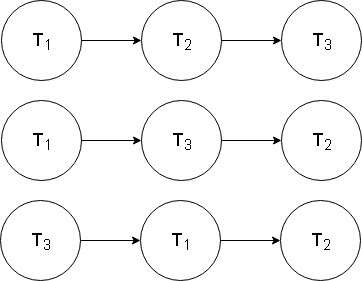
\includegraphics[width=0.5\columnwidth]{h2.png}
	\caption{SG($H_2$)}
\end{figure}

All 3 graphs are possible serialization graphs, with the requirement that $T_2$ follows $T_1$.
\\ \\
\textbf{2PL:}
\\ \\
History 2 above follows 2PL as each transaction adheres to the concurrency protocol by following both the \textit{growing} and \textit{shrinking} phases. However, this history does not follow strict 2PL, as it releases its write locks before the transaction is committed.

\end{document}